\begin{chapter}{Introdução}
\vspace{-0.5cm}
\section{Contextualização}
%página 1
Grande parte das tecnologias disponíveis no mercado já estão economicamente
acessíveis para uma grande parte da população. O uso de dispositivos
eletrônicos, como os \textit{smatphones} e os computadores pessoais, para o
auxílio de diversas tarefas tornou-se mais recorrente no cotidiano das pessoas.
Portanto, com mais pessoas utilizando essas ferramentas, inúmeras formas de
melhorar a interação entre usuários e aparelhos eletrônicos estão surgindo. %ok

O desenvolvimento tecnológico alcançou um estágio no qual a comunicação entre
pessoas e sistemas computacionais está incrivelmente se assemelhando, por
exemplo, com a comunicação estabelecida entre duas pessoas. Graças às diversas
pesquisas realizadas na área da interação humano-computador (IHC) e inteligência
artificial, as máquinas estão se aproximando do comportamento humano no sentido
de serem capazes de executar tarefas semelhantes as ações de ouvir, entender,
pensar e agir de forma automática e independente. %ok

Apesar de todas as melhorias obtidas pela comunidade de pesquisa, as chamadas
interações convencionais~\cite{Preece15} ainda são as mais utilizadas para
controle de dispositivos. Por exemplo, \textit{mouse} e teclado são os
dispositivos de entrada mais utilizados em computadores \textit{desktop}, ao
passo que as telas sensíveis ao toque (\textit{touchscreen}) são utilizados em
\textit{smartphones} e \textit{tablets}. No entanto, esses métodos de entrada
convencionais forçam o usuário a utilizar as mãos, o que se torna um problema
sério se o usuário, por exemplo, possuir algum problema na realização de
movimentos dos membros superiores, o que inclui também pessoas com problemas em
habilidades motoras finas, como fraqueza dos dedos, cujas limitações se
concentram no manuseio de objetos físicos. Nesse sentido, as interações
não-convencionais devem ser exploradas a fim de evitar que pessoas com
deficiência motora sejam digitalmente excluídas.  

%página 2
Interações não-convencionais, por definição, ocorrem quando o usuário é capaz de
se comunicar com um sistema computacional utilizando um dispositivo de
comunicação não tão comum, como câmeras, microfones, ou qualquer outro tipo de
sensor para entrada e/ou saída de dados~\cite{Machado10}. Por exemplo, pode-se
utilizar a fala como uma interação não-convencional para realizar uma tarefa de
digitação. Nesse caso, o dispositivo de entrada utilizado como método
convencional para realizar a digitação (normalmente um teclado) precisa ser
substituído por um microfone. Outro bom exemplo é a utilização de uma
\textit{webcam} para capturar os movimentos a cabeça do usuário e convertê-los
em comandos de controle de um televisor, como em~\cite{Batista17}. Dessa forma,
tais equipamentos são utilizados, portanto, como tecnologias assistivas, pois
elas podem ser a única forma para que pessoas com deficiência motora dos
membros superiores possam interagir de forma autônoma com dispositivos
eletrônicos. %ok
 
A Tecnologia Assistiva (TA) é um campo do conhecimento de característica
interdisciplinar dedicado a aumentar a independência e mobilidade de pessoas
com deficiência (PCD), englobando produtos, metodologias, práticas e serviços
que objetivam promover sua autonomia, qualidade de vida e inclusão
social~\cite{cat09}. O termo refere-se à tecnologia que fornece
assistência a pessoas com diferentes tipos e graus de limitação, a fim de
reduzir os efeitos das deficiências e permitindo-lhes participar ativamente das
suas respectivas rotinas. Segundo a Organização das Nações Unidas (UN, do inglês
\textit{United Nations}), os olhares do século XXI deixam de enxergar as PCD
como ``objetos'' de caridade, tratamento médico e proteção social, e passam a
vê-las sob uma nova perspectiva, na qual as PCD são ``sujeitos'' ativos na
sociedade, capazes de reivindicar seus direitos e tomar decisões baseadas em seu
próprio consentimento~\cite{UN07}. %ok

Através da TA é possível reduzir as dificuldades vivenciadas por pessoas que
necessitam de soluções que não as deixem à margem da utilização de aparelhos
eletrônicos. Visando diminuir a exclusão digital imposta às PCD pela
dificuldade ou total incapacidade para manipular certos equipamentos, a
acessibilidade é vista como elemento fundamental para elevar a autoestima e o
grau de independência dessas pessoas. Além disso, as soluções apresentadas
também podem ser úteis para as pessoas sem qualquer deficiência, já que o
controle de equipamentos torna-se mais prático, confortável e
natural~\cite{Wechsung09}. %ok

Nesse sentido, este trabalho buscou desenvolver um acionador externo baseado em
sopro, que foi utilizado como método não-convencional para realizar a ação de
clique do \textit{mouse}. O dispositivo é capaz de realizar uma comunicação
direta com o computador utilizando a interface de áudio P2 Jack, com o auxílio
de um \textit{software} responsável por capturar os sinais de entrada da
interface de áudio e convertê-los em eventos de clique. Dessa forma, a
utilização da interface USB, que necessita de um microcontrolador para realizar
a comunicação entre o dispositivo e computador, não foi necessário, o que
resultou na diminuição do custo de produção do acionador externo proposto. 

Os usuários-alvo em potencial são pessoas com limitações motoras dos membros
superiores, e que tenham o cognitivo preservado. A ideia é que esse público
consiga realizar, através do sopro, os eventos de clique do \textit{mouse},
descartando a necessidade de utilizar as mão para realizar essa ação. Vale
ressaltar que todas as interfaces de programação e pacotes de \textit{software}
utilizados para a criação do dispositivo proposto neste trabalho são
\textit{open-source} ou encontram-se disponíveis livremente na
Internet~\cite{portaudio},~\cite{xlib}.

%página 3
\section{Justificativa}

Segundo dados da Organização Mundial de Saúde (WHO, do inglês \textit{World
Health Organization}), aproximadamente 15\% da população mundial possui algum
tipo de deficiência~\cite{WHO15}. Esse número é realmente expressivo, pois
revela que, em uma população de 7,6 bilhões de pessoas, cerca de um sétimo
(1~bilhão de pessoas) é portadora de deficiência. A WHO também afirma que,
em 2013, 80\% das pessoas com deficiência viviam em países ainda em
desenvolvimento, o que sugere que o predomínio da condição de deficiência está
bastante relacionado com a situação econômica dos países.
  
No Brasil, segundo o censo realizado em 2010 pelo Instituto Brasileiro de
Geografia e Estatística (IBGE), aproximadamente 23,9\% da população (cerca de
uma entre quatro pessoas, um total de 46~milhões de habitantes) declarou ter
alguma deficiência~\cite{tIBGE}. Os dados também mostram que, desse total, quase
7\% (cerca de de 13,2~milhões) apresentam dificuldades motoras. A
Tabela~\ref{tab:ibge} mostra o perfil da população brasileira com deficiência.

\begin{table}[!h]
\centering
\caption{Perfil da população brasileira com deficiência.}
\label{tab:ibge}
%\vspace{-0.25cm}
\def\arraystretch{1}
\begin{tabular}{lccr}
	\hline
	\hline
	\textbf{Deficiência} & \textbf{Descrição} & \textbf{Número de Pessoas} &
\textbf{Porcentagem} \\
	\hline
	Visual    & Cegueira ou dificuldades gerais   & 35.774.392  & 18,754\%  \\
	\textbf{Motora}    & \textbf{Paralisia ou dificuldades gerais}  & \textbf{13.265.599}  & \textbf{6,95\%} \\
	Auditiva  & Surdez ou dificuldades gerais     & 9.717.318   &  5,094\%  \\
	Cognitiva & Problemas mentais ou intelectuais & 2.611.536   &  1,369\%  \\ 
	\hline
	\hline
\end{tabular}
\end{table} %ok

Apesar da atual existência de inúmeros instrumentos voltados para TA, como
cadeiras de rodas e \textit{software} que facilitam a utilização de
computadores, uma grande parcela das PCD ainda não têm acesso a essas
ferramentas. A Organização Mundial de Saúde estima que, em países
subdesenvolvidos, por exemplo, apenas 15\% das PCD têm acesso a essas Tecnologias
Assistivas~\cite{WHO15}. Um fator que pode contribuir para esse cenário são os
altos preços de algumas dessas tecnologias. 

\subsection{Acionadores Externos}

Acionadores externos, dispositivos que permitem as PCD a utilizarem
equipamentos ativados normalmente por botões ou teclados~\cite{tecla}, são um
grande exemplo de ferramentas voltadas para TA que não são acessíveis
economicamente para grande parte da população. Apesar de existirem uma grande 
variedade de tipos e funcionalidades, a média de dos acionadores externos
é bastante alta. A Tabela~\ref{tab:acionadores} mostra os valores comerciais 
de alguns  acionadores externos. 

\begin{table}[!h]
\centering
\caption{Acionadores externos comerciais.}
\label{tab:acionadores}
%\vspace{-0.25cm}
\def\arraystretch{1.05}
\newcolumntype{C}[1]{>{\centering\arraybackslash}p{#1}}
\begin{tabular}{ccC{3cm}cC{3cm}}
	\hline
	\hline
	\textbf{Nome} & \textbf{Ref.} & \textbf{Método de acionamento} & \textbf{Comunicação} & \textbf{Custo (USD)} \\
	\hline
	Big Candy Corn        &~\cite{CandyCorn}        & Aproximação     & P2 Jack      & 215              \\
	%Pal Pad                &~\cite{PalPad}           & Pressão         & P2 Jack      &  48 à 61         \\
	Jelly Bean             &~\cite{JellyBean}        & Pressão         & P2 Jack      &   65             \\
	%Chin Switch            &~\cite{Chin}             & Pressão         & P2 Jack      & 220              \\
	Micro Light            &~\cite{MicroLight}       & Toque           & P2 Jack      & 85               \\ 
	HoneyBee               &~\cite{HoneyBee}         & Aproximação     & P2 Jack      & 149              \\
	AbleNet string Switch  &~\cite{StringSwitch}     & Puxa corda      & P2 Jack      & 65               \\
	Blue2 Switch           &~\cite{Blue2}            & Pressão         & Bluetooth    & 185              \\
	%Savant Elite2          &~\cite{SavantElite2}     & Pressão         & USB          & 38 à 181         \\
	Foot Pedal             &~\cite{FootPedal}        & Pressão         & USB          & 267              \\
	%Foot Switch            &~\cite{FootSwitch}       & Pressão         & USB          & 26               \\
	Sip/Puff Switch        &~\cite{SipPuff}          & Sopro ou sucção & USB          & 319              \\  
	
	\hline
	\hline
\end{tabular}
\end{table}

Acionadores que possuem como saída de comunicação o P2 Jack,
como~\cite{CandyCorn}, ~\cite{JellyBean},~\cite{MicroLight}, ~\cite{HoneyBee}
e~\cite{StringSwitch}, são mais utilizados como chaves para um determinado
circuito, como a ativação da fala programada de uma boneca através do
pressionamento de um acionador~\cite{ATswitchYT}. %Como forma de controle de uma
%determinada função do %computador --- como o clique de um \textit{mouse} ---
%através de um acionador %externo, não foi encontrado nenhum dispositivo que
%utiliza a comunicação P2 Jack %conectado diretamente no computador que realiza
%essa tarefa.  
É possível controlar o clique de um mouse com a comunicação P2
Jack, mas é necessário o auxílio de um \textit{mouse}, como~\cite{MouseJack},
mostrado na Figura~\ref{fig:mouse}, que possua uma adaptação que receba como
entrada o P2 Jack de um acionador.  Já para acionadores,
como~\cite{Blue2},~\cite{FootPedal} e ~\cite{SipPuff}, que possuem comunicação
Bluetooth ou USB, conseguem realizar o controle dos evento de clique de
\textit{mouse} facilmente sem o auxílio de outros dispositivos, bastando apenas
realizar uma pequena configuração no próprio acionador. Todavia, no caso do
Bluetooth, é necessário um computador que possua suporte a tecnologia Bluetooth,
e, inicialmente, é fundamental realizar o pareamento do \textit{mouse} no
computador para conseguir realizar as funções de clique com o acionador. Já no
caso do USB, a interface é realizada somente com o auxílio de um
microcontrolador que possui a função de implementar o protocolo de comunicação
entre o acionador e o sistema operacional do computador.

\begin{figure}[!h]
	\centering
	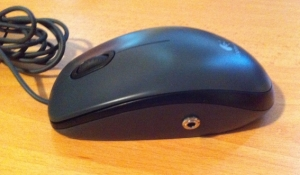
\includegraphics[width=0.65\textwidth]{fig/mouse13}
	\caption{Mouse adaptado para receber a interface P2 Jack de um acionador.}
	\label{fig:mouse}
\end{figure}

Existem também produtos no mercado com a proposta de controlar os eventos de
clique através do sopro, por exemplo, como o acionador Sip/Puff
Switch~\cite{SipPuff} e o IntegraMouse~\cite{IntegraMouse} --- um produto que
permite controlar o ponteiro do \textit{mouse} e realizar cliques no computador,
através dos movimentos da boca e de sopro, respectivamente. Entretanto, o
Sip/Puff Switch custa cerca de U\$ 319, já o IntegraMouse está custando em média
\euro 2000. Esses preços são extremamente altos para pessoas de baixo poder
aquisitivo. Esse alto preço contribui bastante para que esse tipo de TA não seja
amplamente difundida, contribuindo para o aumento da exclusão digital imposta às
PCD.

Como pode ser visto, o custo dos acionadores comerciais são bem elevados. Alguns
deles possuem um mecanismo bem simples e ainda assim são vendidos a valores
absurdos. Por exemplo, o acionador~\cite{StringSwitch} possui apenas uma simples
corda que puxa uma chave de fim de curso. Assim, quando o corda do acionador é
puxada, os pinos de referência e saída do P2 Jack são curto-circuitados,
``simulando'', no P2 Jack, os mesmos estados de aberto e fechado da chave de fim
de curso. Realizando pesquisas em sites como
MercadoLivre\footnote{\url{https://www.mercadolivre.com.br/}}, é possível
encontrar a unidade de uma chave similar a utilizada nesse acionador externo
custando cerca de R\$ 2,50. Já o pino de P2 jack custa cerca de R\$ 1. Com esses
dois materiais é possível construir um acionador semelhante ao discutido
custando menos de R\$ 10, valor bem abaixo dos U\$ 65 cobrado por esse
acionador. %ok

Na atual crise em que o Brasil se encontra, uma família de baixa renda, por
exemplo, dificilmente iria adquirir um acionador externo devido ao elevado custo
desse produto, pois certamente comprometeria sua renda mensal.  Considerando uma
renda mensal de um salário mínimo  (R\$ 954) e o preço do dólar a R\$
3,85~\footnote{Retirado de: \url{https://www.xe.com/pt/} em 17 jul. 2018},
aproximadamente 26\% desse salário seria comprometido para comprar um acionador
de U\$~65. Sendo assim, PCD de baixa renda ficam impossibilitadas de adquirir
tais produtos, excluindo-as de usufruir de dispositivos que são voltados para
facilitar o uso de equipamentos que não são adaptados para esse determinado
público. %ok

Nesse sentido, esta pesquisa tem como intuito apresentar uma solução para
diminuir a exclusão digital vivenciada pelas PCD, que muitas vezes não conseguem
utilizar aparelhos eletrônicos, como \textit{smartphones} e computadores
\textit{desktop}, devido a limitação de recursos que os adaptem às suas
necessidades. Além disso, a solução proposta, apesar de ser voltada para o uso de
uma determinada função em sistemas computacionais, pode ser utilizada em outros
dispositivos que necessitem de uma interação através do pressionamento de um
botão, como ligar ou desligar televisores. Como grande parte dos acionadores
disponíveis no mercado possuem um custo muito elevado, há a necessidade de a
solução proposta ser de baixo custo para que mais PCD possam ter
acesso a essa ferramenta. 

% que %auxiliam o uso de tarefas em dispositivos que normalmente não possuem
% interfaces %alternativas de controle. 
 
\subsubsection {Pesquisas Acadêmicas Relacionadas à Acionadores Externos}

A ideia de ajudar PCD a utilizar aparelhos eletrônicos com o auxílio de
acionadores externos tem sido alvo de inúmeras pesquisas acadêmicas. Uma grande
parte dessas pesquisas foca no auxílio de tarefas de controle das funções
básicas do \textit{mouse} de um computador, onde geralmente se utiliza o
movimento da cabeça ou dos olhos como método não-convencional de controle do
cursor do \textit{mouse}. No entanto, para esse tipo de abordagem, há uma certa
dificuldade em emular a função de clique.  Normalmente, para essa determinada
função,  é utilizada o \textit{dwell time}, um método que utiliza um tempo
específico em segundos em que o ponteiro do mouse fica sobre um determinada área
da tela para realizar  o clique. Todavia, tal técnica obriga o usuário a ficar
com a cabeça ou com os olhos parados em uma determinada posição por algum tempo
para que a função de clique seja ativada, gerando um certo incômodo no usuário.
%,
%além de, naturalmente, aumentar o tempo de utilização a medida em que o número
%de tarefas realizadas também aumentar.

Outro problema recorrente do \textit{dwell time} é esse método naturalmente
demanda mais tempo, em comparação com o método convencional de clique, 
para executar uma tarefa. Devido isso,
há diversas pesquisas que tentam solucionar esses problemas do \textit{dwell
time} através de métodos alternativos para a emulação do clique do
\textit{mouse}.  Em~\cite{Aanand18} foi proposto um algoritmo chamado de
OptiDwell para emular a função de clique.  Esse algoritmo utiliza o mesmo
princípio do \textit{dwelltime}, mas com a diferença de que o usuário sabe
exatamente, através de \textit{feedbacks} visuais e sonoros, quando o evento de
clique irá acontecer.  Com o algoritmo OptiDwell, o usuário tem uma noção mais
precisa do tempo para que a função de clique seja realizada. O usuário sabe que
o clique está para ser realizado através da mudança de cor do cursor do
\textit{mouse}. Por exemplo, se a pessoa deseja clicar em uma letra no teclado
virtual, a cor do ponteiro ficará mudando ao longo do tempo. Quando o ponteiro
estiver em uma determinada cor, a função de clique será chamada, além de ser
ativado um som de estalo (clique). Com isso a pessoa tem uma noção mais precisa do
tempo para realizar o clique, porém o tempo de execução dessa função continua 
sendo um problema.

O trabalho proposto em~\cite{Skim10} utiliza um acionador baseado em dois
componentes ópticos: um LED (do inglês \textit{light emitting diode}) infravermelho
emissor e um receptor. Os LEDs foram posicionados bem próximos a um dos
olhos do usuário e através do valor da tensão no LED infravermelho receptor foi
possível identificar se a pessoa estava de olho aberto ou fechado. Quando o
usuário está de olho aberto , o sinal infravermelho refletido no olho gera uma
tensão bem abaixo da tensão percebida quando a pessoa está com o olho fechado.
Com isso, foi possível detectar os eventos de clique identificando os piscar dos
olhos. A detecção foi baseada na amplitude do sinal de tensão do LED receptor e
no tempo em que o usuário ficava de olho fechado, evitando que o sistema
identificasse um clique de involuntário quando a pessoa piscasse de forma
natural. Esse acionador construído para realizar o clique de um \textit{mouse} é
bastante interessante, porém, como descrito em~\cite{Batista17}, onde foi
elaborado um acionador que utiliza esse mesmo princípio de funcionamento, pode
acarretar uma série de reconhecimentos equivocados de clique devido o sensor
utilizado ser bastante influenciado pelas condições do ambiente, como iluminação
de lâmpadas fluorescentes e do sol.

O método proposto em~\cite{Karimullah02} utilizou o reconhecimento de voz em
inglês para controlar o ponteiro do \textit{mouse} e o evento de clique simples.
Para a movimentação do ponteiro, desenvolveu-se o reconhecimento para cinco
comandos: \textit{move left, move right, move up, move down} e \textit{stop},
para mover o cursor para esquerda, direita, cima, baixo e parar o cursor,
respectivamente. Quando o usuário realiza um comando para mover o cursor,
\textit{move right}, por exemplo, o ponteiro começa a se mover a 20
\textit{pixels} por segundo na direção dado no comando e só para de se
movimentar quando for reconhecido o camando \textit{stop}. Em relação ao evento
de clique, foi implementado apenas o clique simples do \textit{mouse}, sendo
necessário realizar o comando de voz \textit{click} para que o sistema emule
essa função. O trabalho proposto é bastante interessante, mas pode apresentar
problemas, por exemplo, caso o usuário desejar mover o cursor para uma
determinada área que esteja muito próxima da posição atual do ponteiro e não
houver tempo suficiente entre os comandos de mover e parar, o cursor pode não
ficar exatamente sobre a área desejada. Outro grande problema nessa abordagem é
movimentar o cursor na diagonal, pois o usuário é forçado a realizar muitos
comandos de para conseguir posicionar o \textit{mouse} na área desejada.   

Há trabalhos que, para implementar a função de clique, utilizam acionadores
baseados em sinais obtidos por eletromiografia (EMG), um método de registro da
atividade de um músculo quando realiza contração~\cite{Amadio07}.
Em~\cite{Pinheiro12}, por exemplo, foi implementado a função de clique simples e
duplo através de sinais de EMG. Os eletrodos que capturam os sinais elétricos
foram colocados no músculo frontal, conforme mostrado na
Figura~\ref{fig:frontal} Para o clique simples, basta o usuário levantar as
sobrancelhas. Já para o clique duplo, a sobrancelha deve ser levantada duas
vezes de forma consecutiva. Assim, o sinal elétrico capturado pelo circuito de
EMG, quando os músculos da testa são contraídos, é convertido nesses dois
eventos de clique.
  
\begin{figure}[!h]
	\centering
	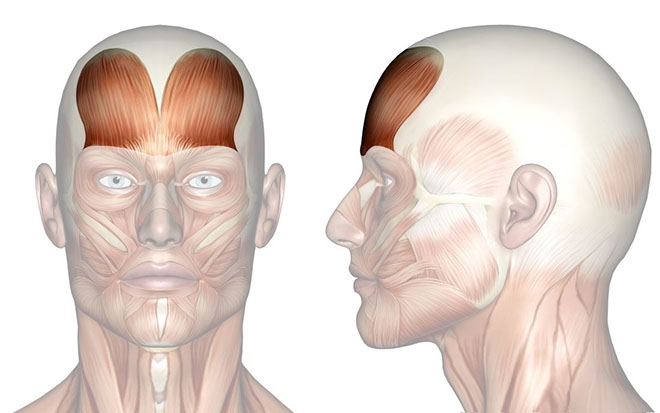
\includegraphics[width=0.5\textwidth]{fig/frontal}
	\caption{Músculo frontal.}
	\label{fig:frontal}
\end{figure}

Já em~\cite{Kaushik12}, foi proposto um acionador que permitia controlar o
movimento do ponteiro do mouse e as funções de clique esquerdo e direito,
através de EMG e mecanomiografia (MMG). A MMG é uma técnica não-invasiva que
registra as vibrações ou sons produzidos pelo músculo esquelético ao se
contrair~\cite{Vaz99}. Os eletrodos de EMG foram colocados nos músculo masseter
e risório, localizados na lateral da face, mostrados nas
Figuras~\ref{fig:masseter} e~\ref{fig:risorio}, respectivamente. 

%Parao MMG foi utilizado um

%%casso
%\begin{figure}
%\centering
%\begin{subfigure}{.4\textwidth}
%  \centering
%  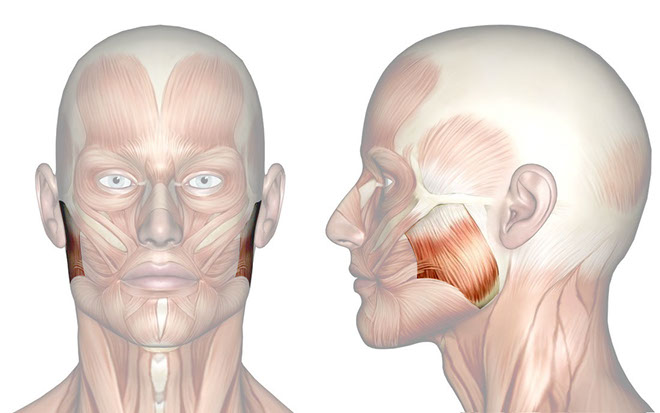
\includegraphics[width=1\linewidth, height=0.2\textheight]{fig/masseter}
%  \caption{Músculo masseter.}
%  \label{fig:masseter}
%\end{subfigure}%
%\begin{subfigure}{0.4\textwidth}
%  \centering
%  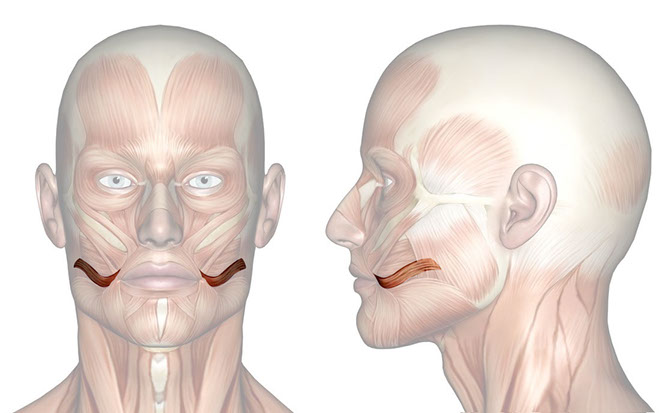
\includegraphics[width=1\linewidth, height=0.2\textheight]{fig/risorio}
%  \caption{Músculo risóro.}
%  \label{fig:risorio}
%\end{subfigure}
%\caption{Músculos localizados na lateral da face.}
%\label{fig:test}
%\end{figure}

\begin{figure}
	\centering
	\subfloat[Músculo masseter.\label{fig:masseter}]{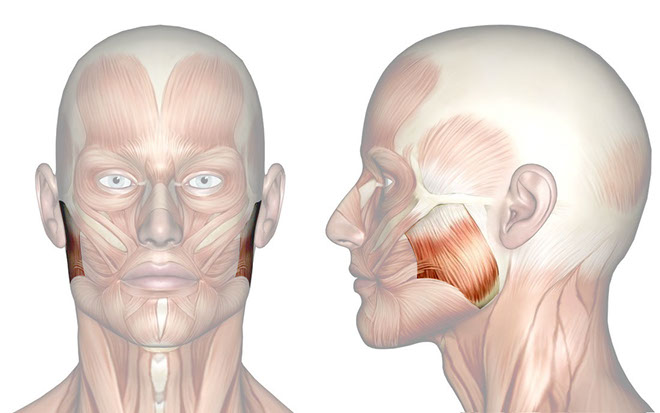
\includegraphics[width=0.48\linewidth]{fig/masseter}}
	\quad
	\subfloat[Músculo risório.\label{fig:risorio}]  {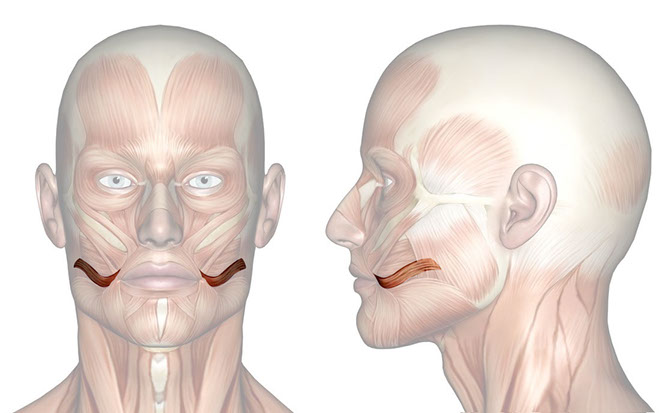
\includegraphics[width=0.48\linewidth]{fig/risorio}}
	\caption{Músculos localizados na lateral da face.}
	\label{fig:test}
\end{figure}

\break
Para o MMG, foi utilizado um piezo --- um transdutor que sob estresses
mecânicos, como vibrações e compressões, gera sinais elétricos --- o qual foi
colocado no músculo platisma localizado no pescoço, como mostrado na
Figura~\ref{fig:platisma}. As palavras \textit{up, down, left} e \textit{right}
foram usadas para mover o ponteiro do \textit{mouse} para cima, baixo, esquerda
e direito, respectivamente. Já para a função de clique esquerdo e direito, foram
utilizadas as palavras \textit{left click} e \textit{right click},
respectivamente. Entretanto, assim como~\cite{Karimullah02}, é preciso realizar
vários comandos para mover o cursor nas diagonais, por exemplo.
\begin{figure}[!h]
	\centering
	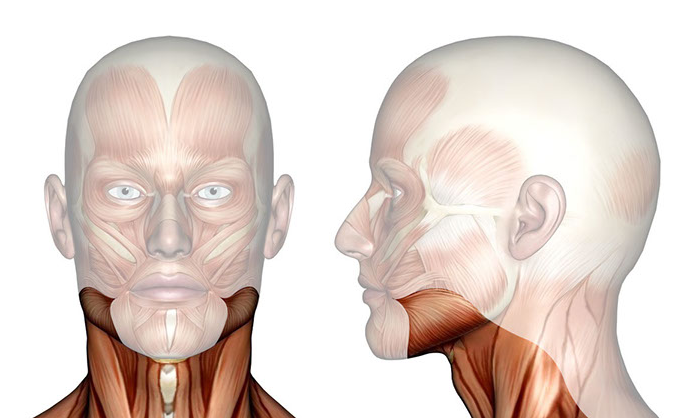
\includegraphics[width=0.5\textwidth]{fig/platisma}
	\caption{Músculo platisma.}
	\label{fig:platisma}
\end{figure}

O trabalho~\cite{Simpson08} realizou o controle do ponteiro através dos
movimentos da cabeça e utilizou um acionador muito interessante que
utilizava os sinais de um acelerômetro para realizar os eventos de clique. O
sensor de aceleração foi posicionado atrás da orelha do usuário, de modo
semelhante como ficam posicionados alguns aparelhos que ajudam pessoas que
possuem dificuldade de audição a melhorar sua capacidade auditiva. Esse
acionador é dividido em dois módulos: transmissor e receptor. O módulo
transmissor é o que fica, de fato, posicionado atrás da orelha do usuário. Já o
receptor fica conectado diretamente no computador via USB. Os módulos se
comunicam utilizando sinais de rádiofrequência. Para ativar a função de clique,
o usuário deve realizar uma pressão entre os dentes superiores e inferiores
(oclusão).  O sensor é capaz de distinguir o comando de clique através da
pressão entre os dentes, da vibração causada no sensor quando o usuário
movimenta a cabeça e até mesmo da vibração causada pelo ato de abrir a boca ao
falar ou bocejar. Isso evita que cliques sejam detectados de forma equivocada,
tornando o acionador mais confiável para o função do clique.

No trabalho desenvolvido em~\cite{Antunes16}, os movimentos da cabeça capturados
por uma \textit{webcam} foram utilizados para controlar o ponteiro do mouse. Já
o evento de clique é realizado com auxílio de um acionador baseado em pressão,
do tipo pedal, bem semelhante aos pedais utilizados por guitarristas para
realizar distorções em notas musicais. O acionador possui uma comunicação direta
com o computador através da tecnologia Bluetooth. Com isso, uma pessoa que tenha
os movimentos dos membros inferiores preservados, consegue utilizar a função de
clique no computador sem a necessidade de utilizar a mãos. 

O FlipMouse, descrito em~\cite{Aigner16}, permite que uma pessoas controle o
cursor do \textit{mouse}, bem como a função de clique. Um módulo
\textit{joystick} e seu \textit{switch} são utilizados para mover o cursor e 
realizar o clique esquerdo, respectivamente. Já o clique direito do
\textit{mouse} é realizado com um auxílio de um microfone de eletreto que é
responsável por detectar o sopro realizado pelo usuário. A comunicação entre o
FlipMouse e o computador é estabelecida através da interface USB com o auxílio
de um microcontrolador que gerencia o protocolo de comunicação exigida pela
interface USB.

Como visto até agora, existem diversos tipos de acionadores construídos com a
finalidade de serem utilizados como método alternativo para o clique do
\textit{mouse}.  Contudo, dentre a literatura consultada, apenas o FlipMouse
desenvolveu um dispositivo que permite realizar algum evento de clique através
do sopro do usuário. Até existem pesquisas na área acadêmica que desenvolveram
acionadores baseados em sopro, como~\cite{Thaller13},~\cite{Mougharbel13}
e~\cite{Filho14}, porém nenhum desses dispositivos são utilizados como interface
para gerar comandos de clique para serem emulados no computador. Já acionadores
que conseguem controlar alguma funcionalidade do \textit{mouse}, 
como os descritos anteriormente,  realizam a comunicação com o computador 
através da interface USB ou Bluetooth, aumentando o custo de desenvolvimento do
dispositivo. Os acionadores que possuem o P2 Jack como interface de comunicação 
não conseguem controlar uma função do \textit{mouse} diretamente através da
interface de áudio do computador. Um \textit{software driver} para capturar os
sinais de áudio e convertê-los em eventos de clique, por exemplo, seria
necessário e uma proposta semelhante a essa não foi encontrada.    


%Diante de tais circunstâncias, este trabalho tem como finalidade apresentar  uma
%solução para diminuir a exclusão digital vivenciada por PCD, as quais estão à
%margem do mundo eletrônico por conta da ausência de recursos que adaptem os
%dispositivos às suas necessidades. Sendo assim, um acionador externo baseado em
%sopro facilitaria o uso das funções de clique do \textit{mouse} para tarefas
%executadas no computador e essa ferramenta seria utilizada em conjunto, por
%exemplo, com um \textit{software} que capture imagens do rosto do usuário em
%tempo real através de uma \textit{webcam} para controlar o movimento do cursor
%do \textit{mouse} ao longo do monitor. Dessa forma, uma pessoa que antes não
%conseguia utilizar um computador, poderá realizar várias tarefas no computador
%forma independente, ajudando na inclusão digital e social dessa pessoa.

Diante de tais circunstâncias, este trabalho tem como finalidade apresentar  uma
solução de baixo custo para diminuir a exclusão digital vivenciada por PCD, 
as quais estão à margem do mundo eletrônico por conta da ausência de recursos 
que adaptem os dispositivos às suas necessidades. Para isso, foi desenvolvido 
um acionador externo baseado em sopro capaz de realizar o clique do 
\textit{mouse} do computador. A utilização do sopro para realizar o clique do
\textit{mouse} foi escolhida, pois é umas das poucas ações que a grande maioria
das pessoas consegue realizar.  Dessa forma, pessoas com diversos tipos de
deficiência, incluindo as com deficiência motora severa dos  membros superiores,
serão beneficiadas por esse dispositivo. A comunicação entre o acionador e o
computador é realizada através da interface de áudio, com o auxílio de um
\textit{software} que possui a função de capturar os sinais do acionador pela
entrada de áudio do computador e convertê-los em clique. O dispositivo
desenvolvido deve ser utilizado em conjunto com alguma ferramenta alternativa de
controle do ponteiro do \textit{mouse}, como as aplicações que utilizam os
movimentos da cabeça do usuário para realizar essa função. 


\section{Objetivos}

O objetivo geral do projeto é construir um protótipo de acionador externo
baseado e sopro que ajude as PCD a controlarem de forma independente os eventos
de clique do \textit{mouse} e também dispositivos de propósito geral que
necessitam de uma interação através de botão ou teclado. A princípio, como prova
de conceito, será possível controlar os cliques, com o auxílio de um
\textit{software driver}, apenas em sistemas operacionais Linux, como o Ubuntu e
seus derivados. No entanto, o sistema projetado pode ser ampliando para os
sistemas operacionais Windows e MacOS para atender um maior número de potenciais
usuários do produto. É importante também que esse produto seja de baixo custo e
que todo o projeto seja livremente disponibilizado% para que qualquer pessoa que
%tenha acesso a esse projeto, se desejar, possa construir por conta própria seu
%acionador, aumentando assim, o número de pessoas beneficiadas por este trabalho.

%O protótipo deve ser colocado em uma posição próxima a boca do usuário com o auxílio
%de um \textit{headset} modificado que servirá de suporte para ajudar o acionador
%a ficar em uma posição ideal para que o usuário consiga realizar o sopro sem
%dificuldades. A interface de comunicação do acionador com o computador será o
%P2 Jack 3.5~mm para que a pessoa possa utilizar o mesmo acionador, que foi
%projetado para usar a função de clique de um \textit{mouse}, em outro tipo de
%contexto, como em brinquedos que precisam de um tipo de acionamento externo. Um
%\textit{software} será desenvolvido para capturar os sinais da interface P2 Jack
%e convertê-los em ações de clique no computador.

%Testes com o protótipo serão aplicados a voluntários para verificar o potencial
%do produto e verificar possíveis desvantagens para futuras melhorias.

\begin{subsection}{Objetivos Específicos}

Os objetivos específicos podem ser:
i) estudo e implementação das ferramentas que constituem acionador;
ii) estudo de APIs para criação do \textit{software};
iii) teste com voluntários;

Uma breve descrição sobre cada tópico é feita a seguir.

\begin{enumerate}[i)]

\setlength\itemsep{-.2cm}
	\item Estudo e implementação ferramentas que constituem o acionador: \vspace{-.2cm}
	\begin{itemize}
		%\setlength\itemsep{-.1cm}
		\item Estudo de componentes eletrônicos sensíveis ao fluxo de ar
provocados pela ação de sopro.
	\end{itemize}

	\item Estudo de APIs para a criação do \textit{software}: \vspace{-.2cm}
	\begin{itemize}
		%\setlength\itemsep{-.1cm}
		\item Estudo de APIs para captura de sinais da interface P2 Jack;
		\item Estudo de APIs que permitam manipular os eventos de clique;
		%\item Implementação do \textit{software}.
	\end{itemize}

	\item Testes com voluntários: \vspace{-.2cm}
	\begin{itemize}
		%\setlength\itemsep{-.1cm}
		\item Definição de um cenário de testes compostos pelo método proposto 
		e outro método alternativo para os eventos de clique;
		\item Aplicação de um questionário capaz de quantificar atributos 
		qualitativos do sistema.
	\end{itemize}


\end{enumerate}

\end{subsection}

\section{Síntese de Conteúdos}

Este capítulo fez uma breve introdução sobre as motivações que levaram ao
desenvolvimento do projeto além de mostrar os objetivos do trabalho.
A seguir, é apresentada uma síntese dos conteúdos que serão abordados nos
próximos capítulos.

\begin{description}
	\item[Capítulo 2.] Revisão Teórica.
	Uma introdução das principais ferramentas para o desenvolvimento do trabalho
será feita. Serão abordados tópicos sobre piezoeletricidade; amplificadores
operacionais; Conectores de áudio; ferramenta de desenvolvimento de placa de
circuitos impressos; Captura de áudio através da interface P2 Jack; Ferramentas
para emulação de cliques do \textit{mouse}. 

	\item[Capítulo 3.] Metodologia. 
	Neste capítulo, as atividades realizadas para a construção do projeto serão
	detalhadas. Serão descritos com detalhes os procedimentos utilizados
	para que o acionador construído pudesse se comunicar com o computador
	através da interface P2 Jack com o auxílio do \textit{software} desenvolvido,
	o qual é capaz de capturar os sinais do P2 Jack e convertê-los em ações de
	clique.
	
	\item[Capítulo 4.] Ambiente de Teste e Resultados. 
	O sistema foi testado com algumas pessoas, as quais forneceram um
	\textit{feedback} através de um questionário de qualidade baseado em uma escala
	quantitativa.  Os detalhes sobre a metodologia dos testes aplicados aos voluntários e
	os resultados obtidos e avaliados. Detalhes sobre as falhas cometidas e
	dificuldades gerais encontradas durante o projeto também serão relatados neste
	capítulo.

	\item[Capítulo 5.] Considerações Finais. 
%	Discussões sobre os resultados dos testes feitos com o grupo de voluntários
%	serão abordadas nesse capítulo, 
    Neste capítulo será apresentado a conclusão do trabalho, as contribuições do
	projeto e a perspectiva para as próximas versões do dispositivo, esta última 
	discutida na seção de trabalhos futuros. 

	%DDDetalhes sobre todas as falhas cometidas e
%	dificuldades gerais encontradas durante o projeto também serão relatados. 
\end{description}

\end{chapter}
